\documentclass[times, twocolumn]{article}
\usepackage{graphicx} % Required for inserting images
\usepackage{subcaption}
\usepackage{amsmath}
\usepackage{float}
\usepackage{pgfplots}
\usepackage{subcaption}
\usepackage{comment}
\usepackage[a4paper, total={7in, 9in}]{geometry}
\usepackage{biblatex}

\addbibresource{mybib.bib}

\title{Spotify Tracks Genre Classification}
\author{Nabeha Barkatullah, Mia Striebeck, Laksha Karthikeyan, Carson Chiem, Shuzo Naruse}
\date{May 20, 2024}

\begin{document}
\maketitle

\newpage
% abstract
\begin{abstract}
Discovering new music that fits within your music taste is time-consuming and difficult. On top of there being an abundance of music to sift through, finding songs from the bulk that you actually enjoy listening to can go either way. With this project, we aim to utilize a Spotify dataset to build a model to classify songs under genres, with the potential of being part of a song recommendation system. Using the attributes from the dataset, such as the relevant music listening patterns and classification of songs, we will predict the genre a song falls under. Our goal is to build a classification model that predicts a song’s genre based on user-inputted track features.
\end{abstract}
\section{Introduction}
With music production becoming increasingly accessible, music platforms have subsequently become saturated with new music. For newer or more niche artists, being discovered among a sea of other songs and competing within the platform’s algorithm. On the other hand, for users looking for new music, breaking beneath the surface of more popular songs within genres they may enjoy can prove to be difficult and sifting through songs to curate their music profile is time consuming and frustrating when you are not exactly sure what you are looking for. 

This project is posed to be a part of a larger music recommendation system; this aspect of the system encompasses a machine learning driven genre classification model using the K-nearest neighbors method. To narrow down the scope of this project, we have our tool limited to music on Spotify’s platform for data feature accessibility— music uploaded to Spotify has an associated song ID, among other descriptive features about the song. Using Spotify music data sourced from Kaggle, a machine learning model based on K-nearest neighbors was trained and connected to the front end of a web based GUI.  In terms of the front end interaction, the user is able to navigate through our GUI which searches though a Spotify dataset in order to input a song from search and predict the genre it belongs to. As a part of a larger product, this model would be used in tandem with other tools to fine tune a recommendation system based upon other aspects apart from genre. 

For the task of genre classification, machine learning appeared to be the obvious approach due to the apparent degree of subjectivity of the task— the classification of a song into a genre is not always a clear choice but a decision can be made based upon patterns in music. ML is especially useful in this case where genre patterns can help form clearer decision boundaries. Additionally songs often do not belong to one single genre— more often than not they belong to multiple genres such as “Pop, Rock, EDM”, “Indie, Pop”, “Country, Jazz”. With this in mind, utilizing K-nearest neighbors as an ML approach provides a robust solution for the proposed task of genre classification as it provides a cluster of genres that most closely fit the inputted song.  

% background
\section{Background}
The purpose of this project is to lay the foundation for a robust music recommendation system outside of popular platforms music boosting algorithms. While effective, music algorithms within the app have a tendency to push surface level music within genres, often excluding more niche songs within genres— prioritizing breadth over depth in recommendations. While recreational in nature, utility for this tool was immediately recognized among our group as a result of music being so pervasive through the college student experience. 

This project was developed with respect to other existing recommendation systems in our literature review. Spotify has publicly provided open source music data sets with 20 features for use online through Kaggle, as well as web tools for developers. A machine learning approach was integrated into the goals of this project, with methods such as K-NN, random forest, and others considered. 

The use of the  K-NN algorithm was motivated primarily by the targeted functionality of the tool and the adaptability of K-NN as a method. Assigning clusters of applicable genres to a user inputted song seemed relevant for real-life usage since songs are not limited to a single genre. 
%literature review
\section{Literature Review}
Many previous works have utilized machine learning techniques to classify music by genre. R. Prajwal and Sharma et al. (2021) built multiple classification models based on features extracted from audio samples, such as spectral centroid (the weighted mean of the sound frequencies) and the shape of sound signals~\cite{Singhal2022}. They conducted feature selection and hyperparameter tuning using GridSearchCV and RandomizedSearchCV, optimizing the k value for k-NN to maximize accuracy~\cite{Singhal2022}. The models implemented included k-Nearest Neighbors (KNN), Support Vector Machine (SVM), Logistic Regression, and Random Forests~\cite{Singhal2022}. SVM achieved the highest accuracy of 76.4\%, followed by Random Forests with 69.6\%, KNN with 66.4\%, and Logistic Regression with 67.2\%, all after hyperparameter tuning~\cite{Singhal2022}.\\

While their dataset utilized technical audio features such as zero-crossing rate and mel-frequency cepstrum coefficients, our dataset includes numerical measures of musical elements and human interpretations of music, such as the mode, which describes the mood of a song. This is more similar to the work by Rahul Singhal and Shruti Srivatsan, who noted that classification models using Extreme Gradient Boosting and Random Forest performed the best compared to traditional ML approaches~\cite{prajwal2021music}. In particular, a hyperparameter-tuned Random Forest classifier achieved high accuracy and F1-score~\cite{prajwal2021music}.\\

Given that our dataset encompasses features like popularity, acousticness, and danceability, we wanted to explore how Random Forest would perform for our model. The KNN algorithm is noted for its simplicity in terms of workings and calculations. It offers flexibility for various modifications to overcome limitations, enhance accuracy, and increase its applicability to a wider variety of datasets. KNN's adaptability allows for performance improvements through optimizing the k parameter, refining distance calculations, and adding weights to different data points.

\section{Dataset Description and EDA}
\subsection{Dataset Description}
The original Kaggle dataset contains data on Spotify songs from over 125 genres, with each song having associated features related to identification of each track, audio characteristics, or popularity and genre classifications. The original data set contained around 114k rows (songs/tracks) condensed in a CSV format, with 20 features, which are track id, artist name, album name, track name, popularity, duration (ms), explicit, danceability, energy, key, loudness, mode, speechiness, acousticness, instrumentalness, liveness, valence, tempo, and time signature. In efforts to improve our model performance, we also utilized another identical, but larger, dataset from Kaggle, which had the identical features and genres, but with 1 million rows/tracks. This larger dataset was also already cleaned, containing no missing values or duplicate rows, unlike the smaller dataset. To further describe the features, popularity is the ranking of each song on a scale of 1 to 100, duration of the track is in milliseconds (ms), explicit is a boolean value, stating if a song contains explicit lyrics, danceability is a level, from 0 to 1, of a song being considered suitable for dancing, energy is a measure, from 0 to 1, of intensity, key is in regards to overall musical pitch, loudness is measured in decibels (dB), mode indicates if the track is on a major or minor scale (1 or 0), speechiness measures, from 0 to 1, the level of spoken words in a track, acousticness is a measure, from 0 to 1, of instruments used without electrical amplification, instrumentalness is a measure, from 0 to 1, of a track containing vocals, liveness is the likelihood of a song being performed in front of an audience, valence measures the interpretation of a song as positive or negative, tempo is the speed of a track, measured in beats per minute (BPM), and time signature indicates the number of beats in each measure of the piece. All are continuous variables, except for track id, artist name, album name, track name, explicit, popularity and track genre, which are categorical. Popularity is particularly ordinal categorical, as tracks are assigned a ranking of popularity. 

In pre-processing the smaller dataset, we checked for duplicate rows and missing values. 32,656 rows were dropped, as they were each identified as having the same track name and artist as another track. The remaining rows of distinct tracks were filtered to identify missing values for each feature, which identified one track having 3 missing values. Furthermore, the genre feature originally contained 125 classes, however, as many genres were more specific sub-genres, these sub-genres were grouped under their respective overall genres. Both datasets were ultimately subset to only contain tracks of the 10 most popular genres, which are  removing the rows of all other genres. Thus, the resulting cleaned dataset contained 81,344 rows of distinct tracks.

\subsection{Exploratory Data Analysis}
We conducted exploratory data analysis in order to further investigate the distributions of the features in our dataset and their correlations with each other, to identify potential presence of multicollinearity or imbalances in the feature distributions, to help perform feature selection and identify the ten most frequent genres in this dataset.

Figure \ref{graph:dists} shows frequency distributions of the features, showing that the danceability and tempo features have nearly normal distributions, while the distribution of loudness is left-skewed, and acousticness, speechiness, liveness are right-skewed. This signifies that while most of the songs in this dataset are moderately loud, there are some that have particularly low levels of loudness, that makes the distribution skew to the right. Similarly, acousticness, speechiness and liveness have similar levels among most of the songs, although there are some outlier songs with significantly higher levels of acousticness, speechiness and liveness that cause these distributions to skew to the right.

% adding Figure 1 - image of feature distributions
\begin{figure}[H]
    \centering
    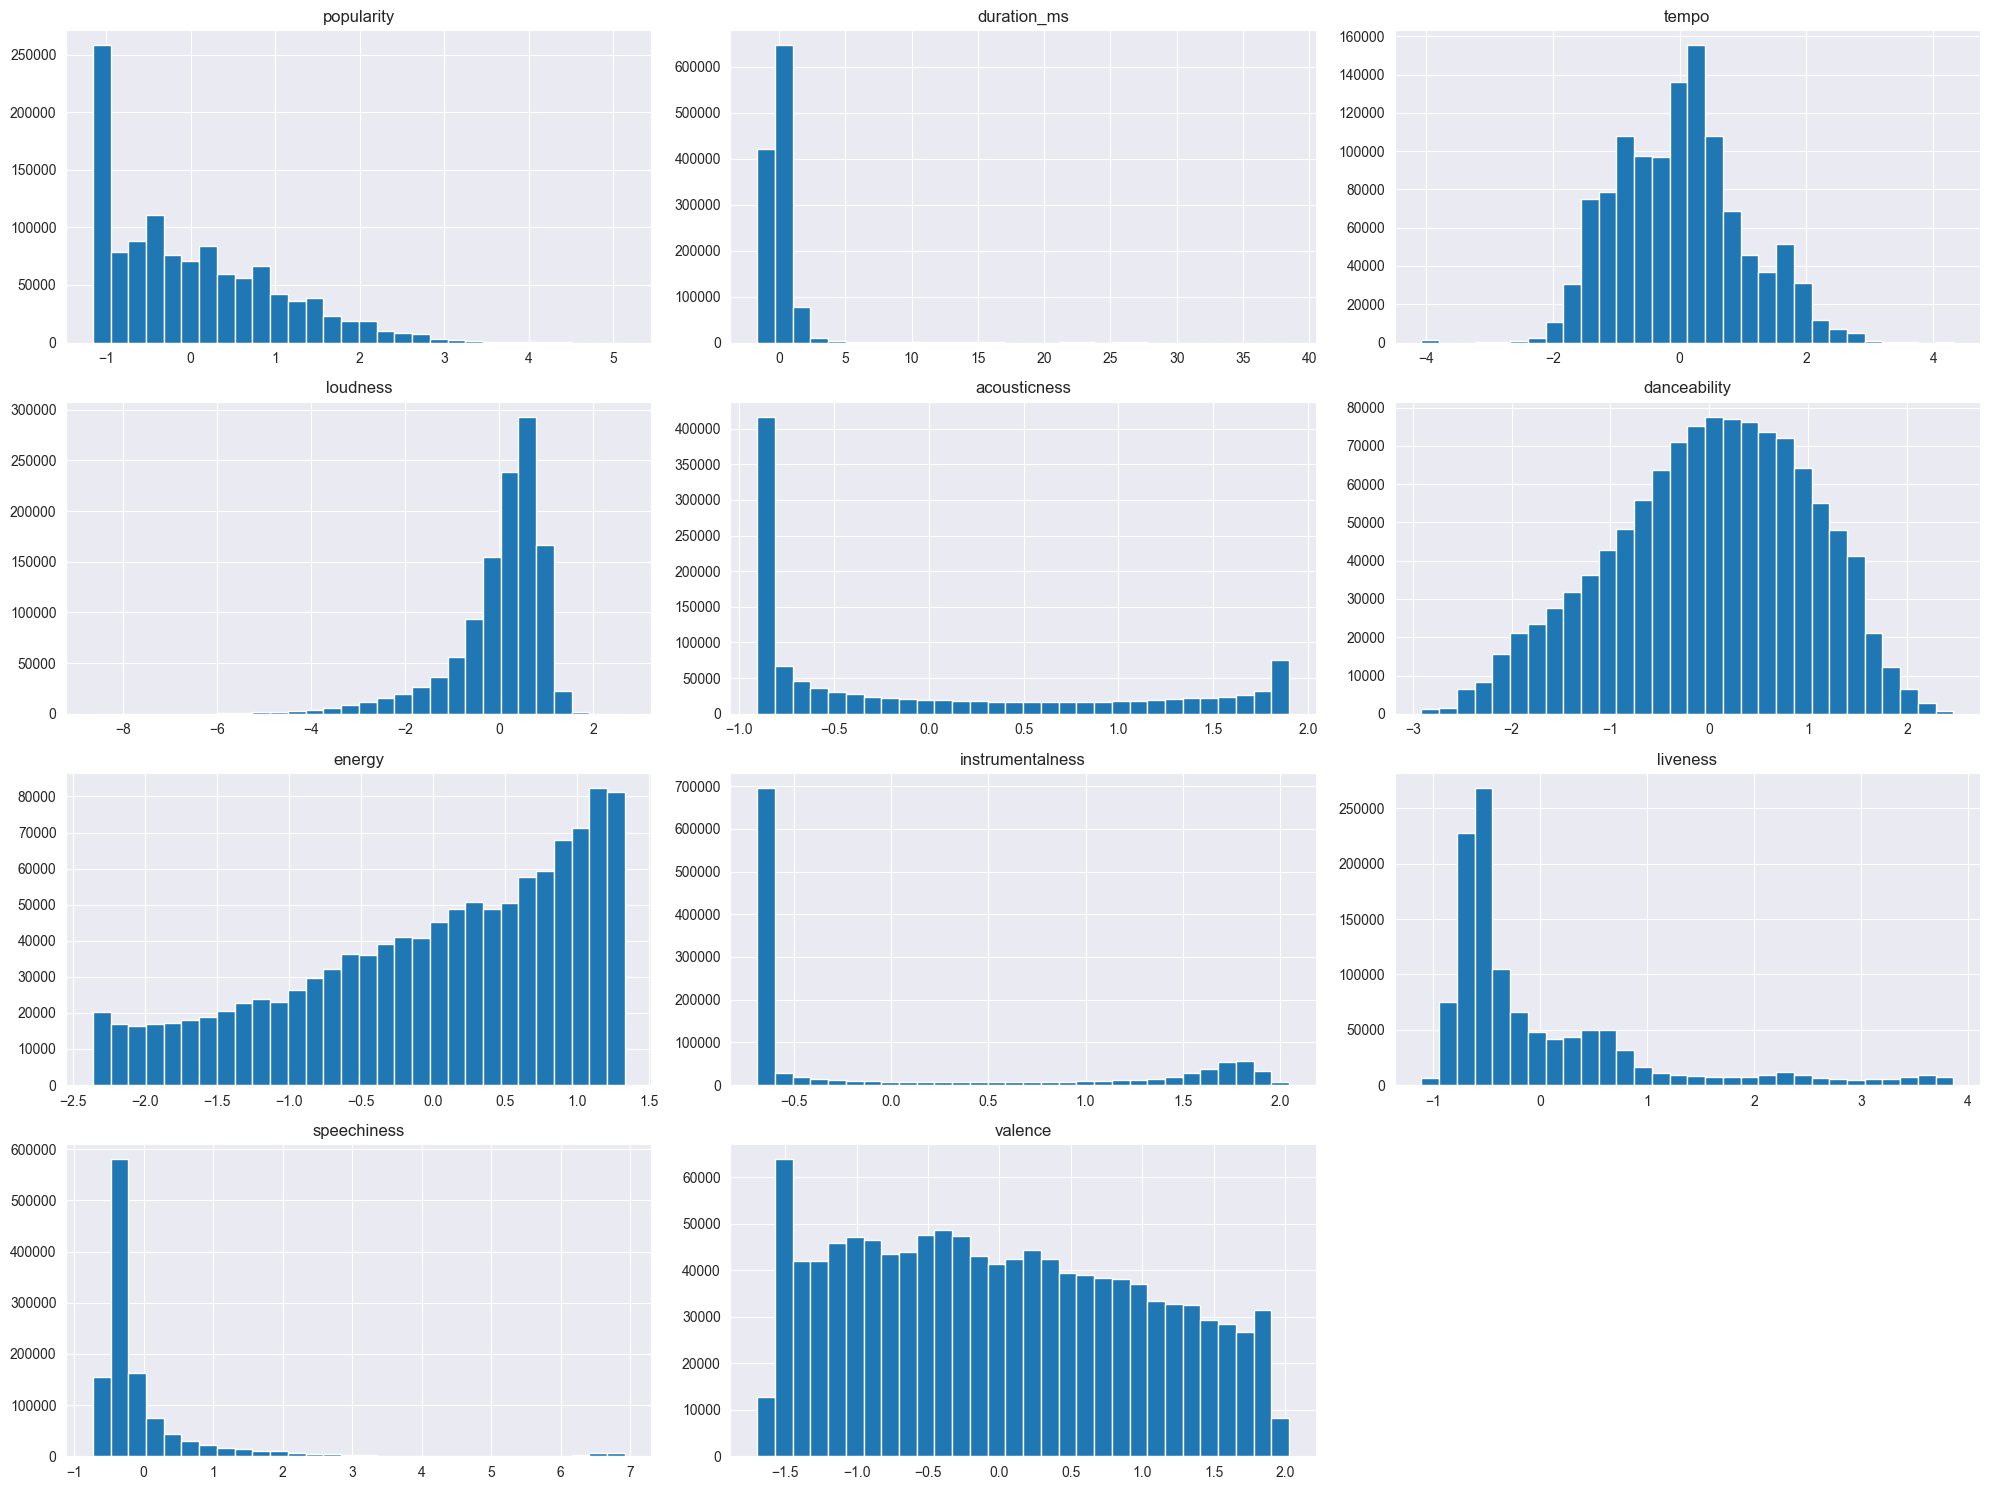
\includegraphics[width=0.55\textwidth]{report_pics/feature_dists_new.png}
    \caption{Frequency distributions of the continuous track features, which have been scaled using z-score normalization.}
    \label{graph:dists}
\end{figure}

Box plots were used to further examine the distributions and identify outliers, as seen in Figure \ref{Boxplots}, which maps the distributions for the ordinal categorical predictor variable popularity, and every continuous predictor variable, which include duration, tempo, loudness, acousticness, danceability, energy, instrumentalness, liveness, speechiness and valence. From this visualization, it is evident that popularity, acousticness, energy and valence have no outliers, while all other features do, although it is expected that popularity contains no outliers, as these are ranked values of a pre-determined range. The presence of outliers is reasonable as it merely shows the diversity of the songs in our dataset, and ultimately, the variety in levels of these features is what characterizes the different music styles that allow a song to be categorized under a certain genre.
% adding Figure 2 - boxplots
\begin{figure}[H]
    \centering
    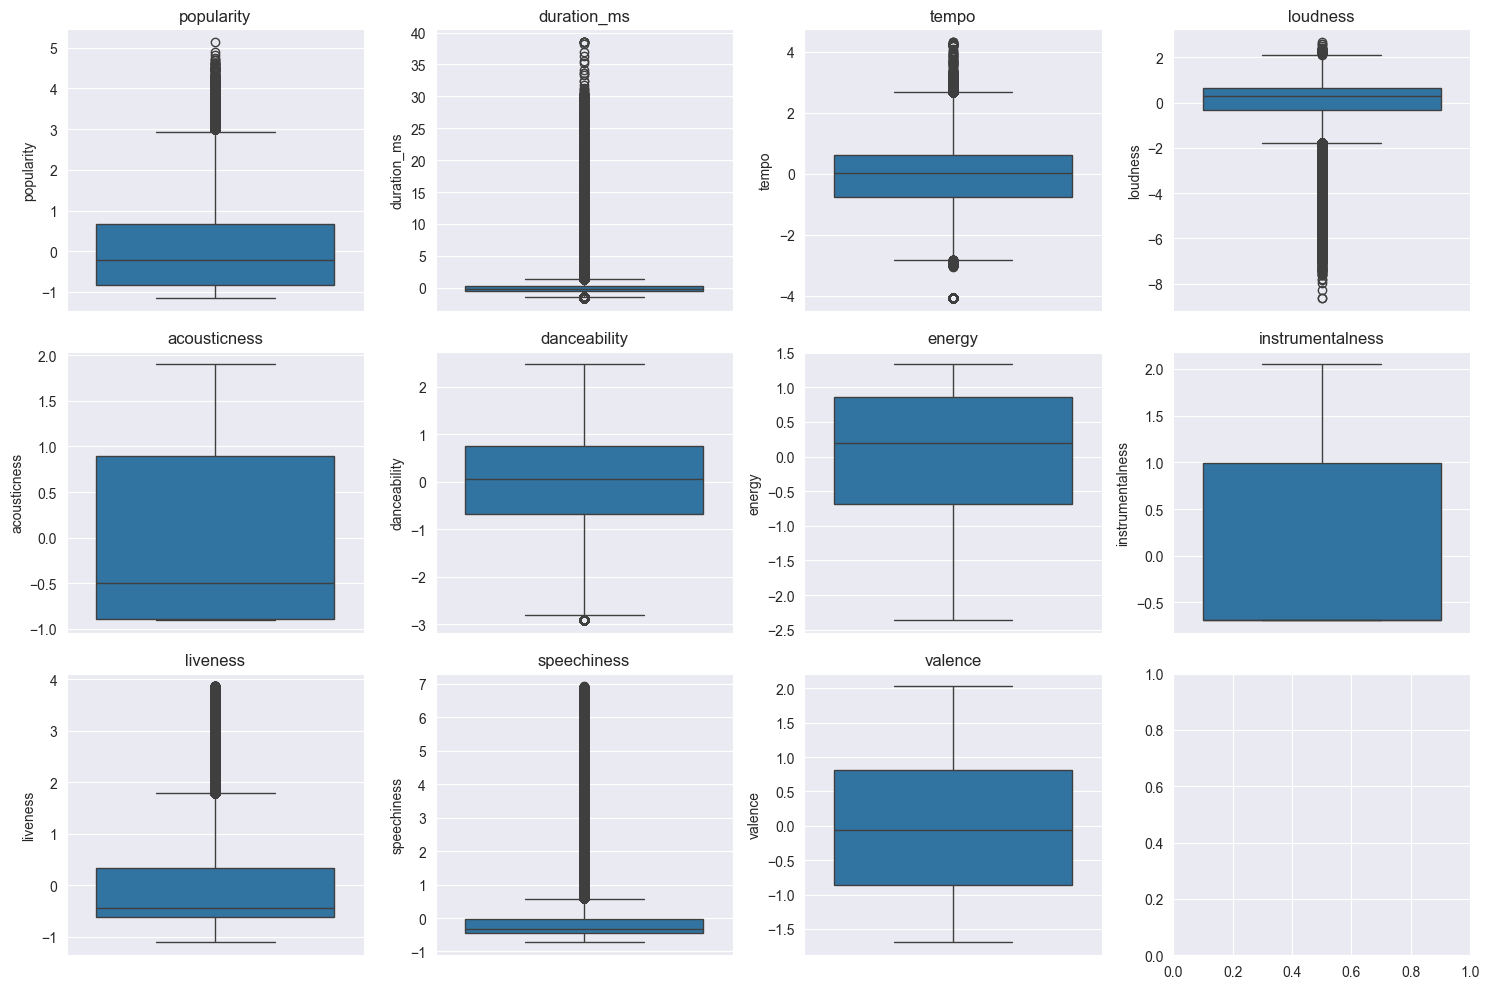
\includegraphics[width=0.5\textwidth, height=10cm]{report_pics/feat_boxplots_new.png}
    \caption{Box plots depicting the distributions of the continuous features in our dataset, scaled using z-score normalization.}
    \label{Boxplots}
\end{figure}
Figure \ref{heatmap} displays the correlations between the continuous predictor variables in the dataset. It shows a significant positive correlation between energy and loudness, and that acousticness is significantly, negatively correlated with both loudness and energy. Further, danceability and valence appear to have a weak positive correlation, and instrumentalness and loudness have a weak negative correlation. Although the significant correlations between multiple features, such as between acousticness with loudness and energy, indicates multicollinearity, it is slight and therefore not likely to have a significant impact on the results of our classification model.
\begin{figure}[H]
    \centering
    \textbf{Pearson's Correlation Heatmap of Relevant Features}
    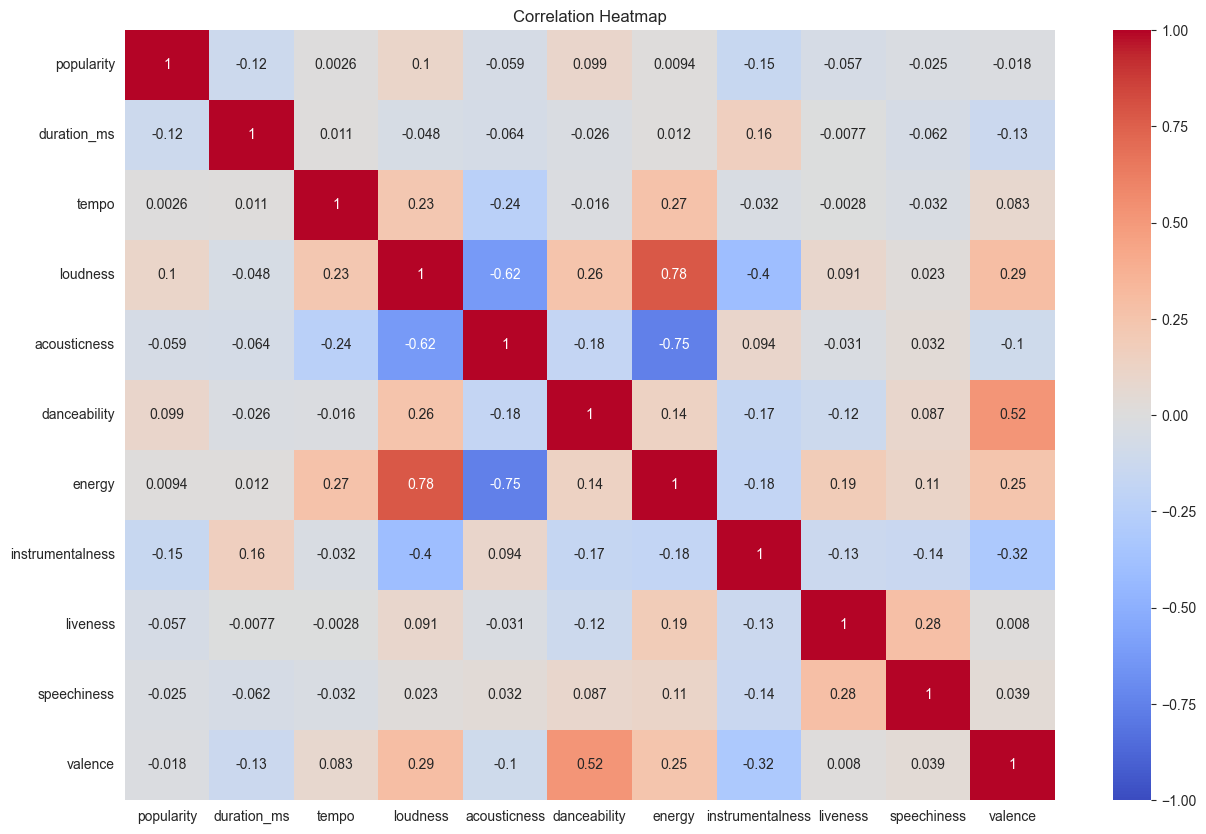
\includegraphics[width=1.0\linewidth]{report_pics/corr_heatmap_new.png}
    \caption{The Pearson's correlation heatmap depicts the pairwise correlations between the 11  continuous features that are relevant to the characteristics of each track, where a value less than 0 indicates negative correlation, and a value greater than 0 indicates positive correlations between the features.}
    \label{heatmap}
\end{figure}

Figure \ref{top10} depicts the 10 most frequent artists and the top 10 most frequent genres that are present in the cleaned dataset. The ten genres with the greatest frequency of tracks in this dataset are Electronic Dance Music (EDM), punk-rock, pop, rock, alt-rock, rock, acoustic, k-pop, classical, piano, and hip-hop, although there appears to be similar frequencies of tracks across these ten genres. Importantly, not all of these most frequent genres are of the 10 most popular genres.

% adding Figure 4 - top 10 most frequent
\begin{figure}[H]
    \centering
    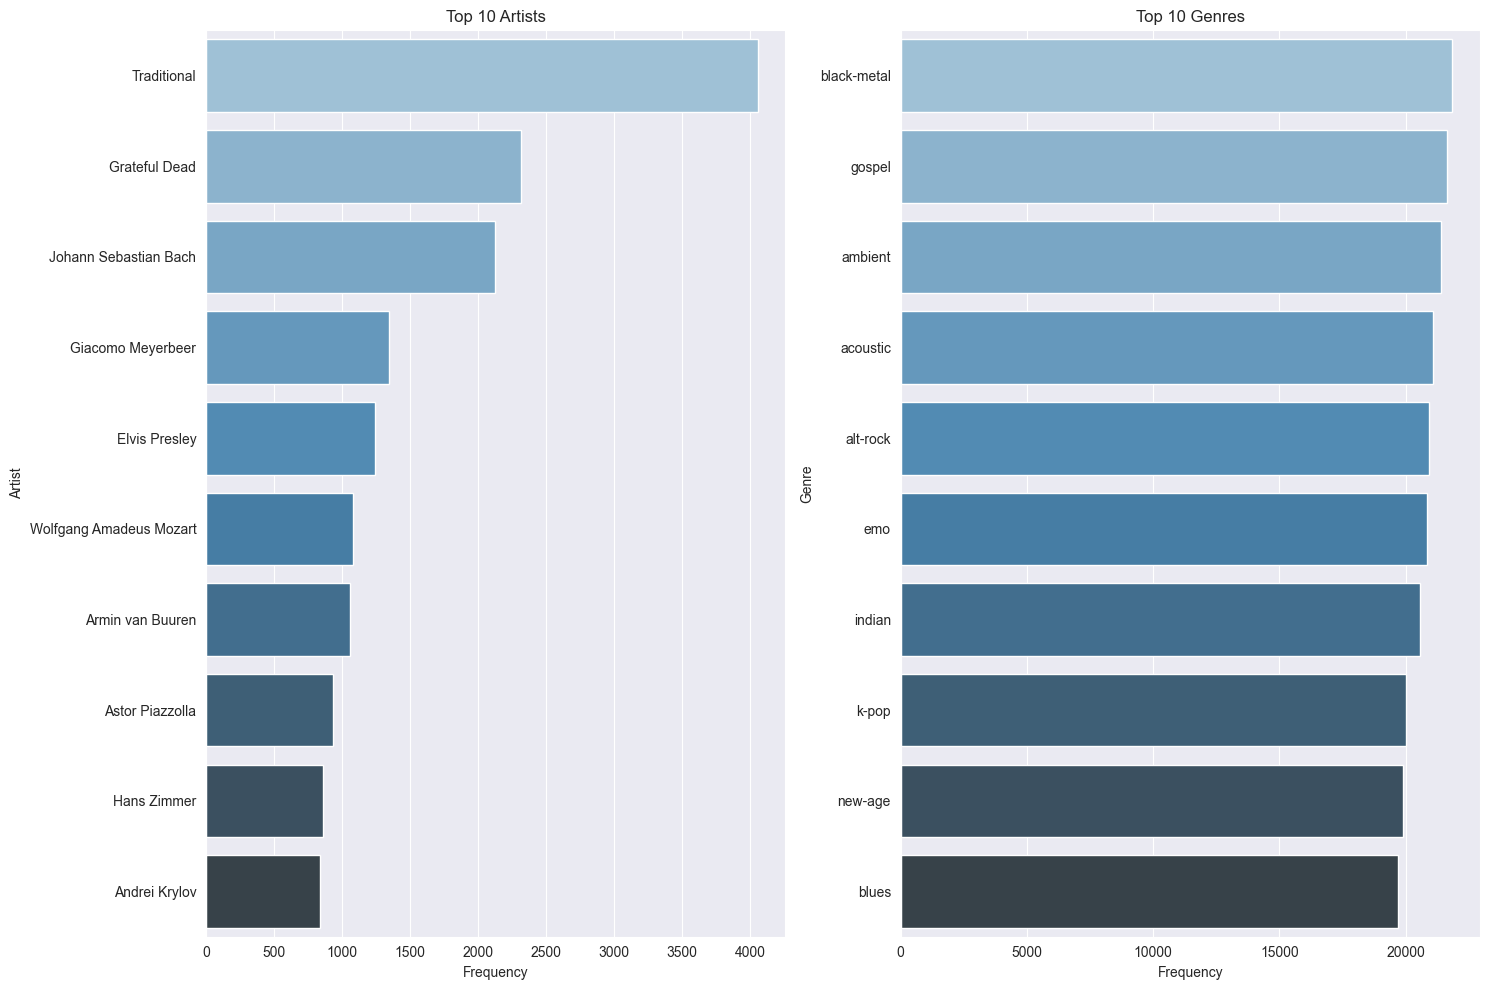
\includegraphics[width=0.5\textwidth]{report_pics/top_genres.png}
    \caption{Top 10 artists and genres}
    \label{top10}
\end{figure}

These results provided useful information in choosing methods that would be best suitable for the characteristics of the dataset, and evaluating the performance of our models, as there were some features with skewed distributions and irregularities in the frequencies of tracks within features, requiring models that are ideally robust to outliers and can capture complex relationships between the features and genre, especially as the analysis indicated slight collinearity between some features, and suitable for a large dataset.

\section{Proposed Methodology}
In order to build a classification model to classify a track to belong to one of multiple genres, based on the predictor variables related to audio characteristics and musical style, we followed the following methodology to identify the most accurate model for our dataset and objective. The smaller dataset was pre-processed, in order to clean the data of missing and duplicate values, to prepare for training the model to our preferences. Feature engineering was then used to identify relevant features, and use those features to build our models, where we implemented Random Forests and k-Nearest Neighbors. \\
 
Our data pre-processing involved identifying and removing duplicate songs from the smaller dataset, as we observed instances where entire rows were duplicated. Additionally, we found cases where the same songs were included more than once under different album names. For example, some songs by The Beatles were included under its original album name, as well as under “best of decade” album. These instances were removed in order to have unique instances for every song during training, mainly to prevent any possible overfitting that may occur if this was not done. There was a single row with 3 missing column values, and it was removed in order to prevent any analysis errors. A large part of our preprocessing involved changing the genre classifications for many songs.  Genres such as “electro”, “trance”,  “techno”,  “idm” and “house” were merged with songs from the “edm” genre in order to create one large group of tracks classified as “edm”, since the aforementioned genres are technically subgenres of electronic dance music. There were other instances of subgenres being included when the umbrella genre is also present such as “rock” and its various subcategories. The genres of “alternative”, “grunge” and “alt-rock" were all merged together, as well as “indie-pop”, “synth-pop”, “dance” and “pop”. By aggregating these genres, the hope was to create larger differences between the possible predictions, with less risk of overfitting, as the model would be less likely to fit too closely to the data of these more specific sub-genres, and a larger sample size within the overall genre would allow for greater accuracy as well.
Feature engineering was done in order to determine the necessary features for our model. From our exploratory data analysis, we gained a solid understanding of our dataset features, as some features were shown to be normally distributed, while others are heavily skewed. The features that had many outliers, such as popularity and duration, were kept because they seemed to have little effect on the accuracy results. This is due to the nature of songs and genres of various musical styles varying in these features, as well as popularity being assigned based on ordered ranking. Other features that did not have numerical data stored, such as key and mode, were encoded using LabelEncoder() into numerical values. Features that were not relevant for genre prediction and were subsequently not used for training included the artist name, track name, track ID, and year of release. \\\\
The feature engineering step as well as how the model was split into training and test sets was the same for smaller and larger datasets. The data was split in training and testing sets by an 80:20 ratio. We initially used a random forest classifier model since previous literature has shown it produced the best results, as well as that it is known to effectively handle a large training set and is robust to outliers as seen in our skewed feature distributions. Hyperparameter tuning using GridSearchCV() was done in order to determine which hyperparameter values were best for our data. However, we pivoted to using K-nearest neighbors in order to get more than one prediction for each track since our accuracy was relatively low for the random forest model at around 50\% using the best hyperparameters. This was after testing our data using both XGBoost and CNN models and having results that were similar or worse. The revised approach was to pick multiple genres that the songs sound similar to, such that a song with features that are close to both “edm” and “pop” will have both listed as output. The nearest neighbors were taken for the inputted song, their genres were counted, and genres outputted that were the most prevalent among the neighbors.\\\\
The metrics utilized to evaluate the performance of the random forest and k-nearest neighbors models were accuracy, precision, recall and F-1 score. The model with the highest accuracy and relevant output was determined the most ideal model.

\section{Experimental Results and Evaluation}
\subsection{Random Forest}
The Random Forest model proved to have a relatively low performance and accuracy, even despite the implementation of XGBoost, which had a slightly lower accuracy result. Figure \ref{rf_confmatrix} summarizes the prediction results through a confusion matrix, from Random Forests without XGBoost. The  diagonal values indicate the true positives for each genre prediction, which is the number of songs with correctly identified genres, compared between the actual and predicted results. It appears that alt-rock, classical and hip-hop were the top three genres with significantly high numbers of true positives, while rock and pop had the lowest number of true positives. As these results are used to calculate performance metric such as accuracy, precision and the F1-score, it reflects on the lower accuracy result of approximately 50\% from the Random Forest model.

% adding Figure 5 - Random Forest Confusion Matrix
\begin{figure}[H]
    \centering
    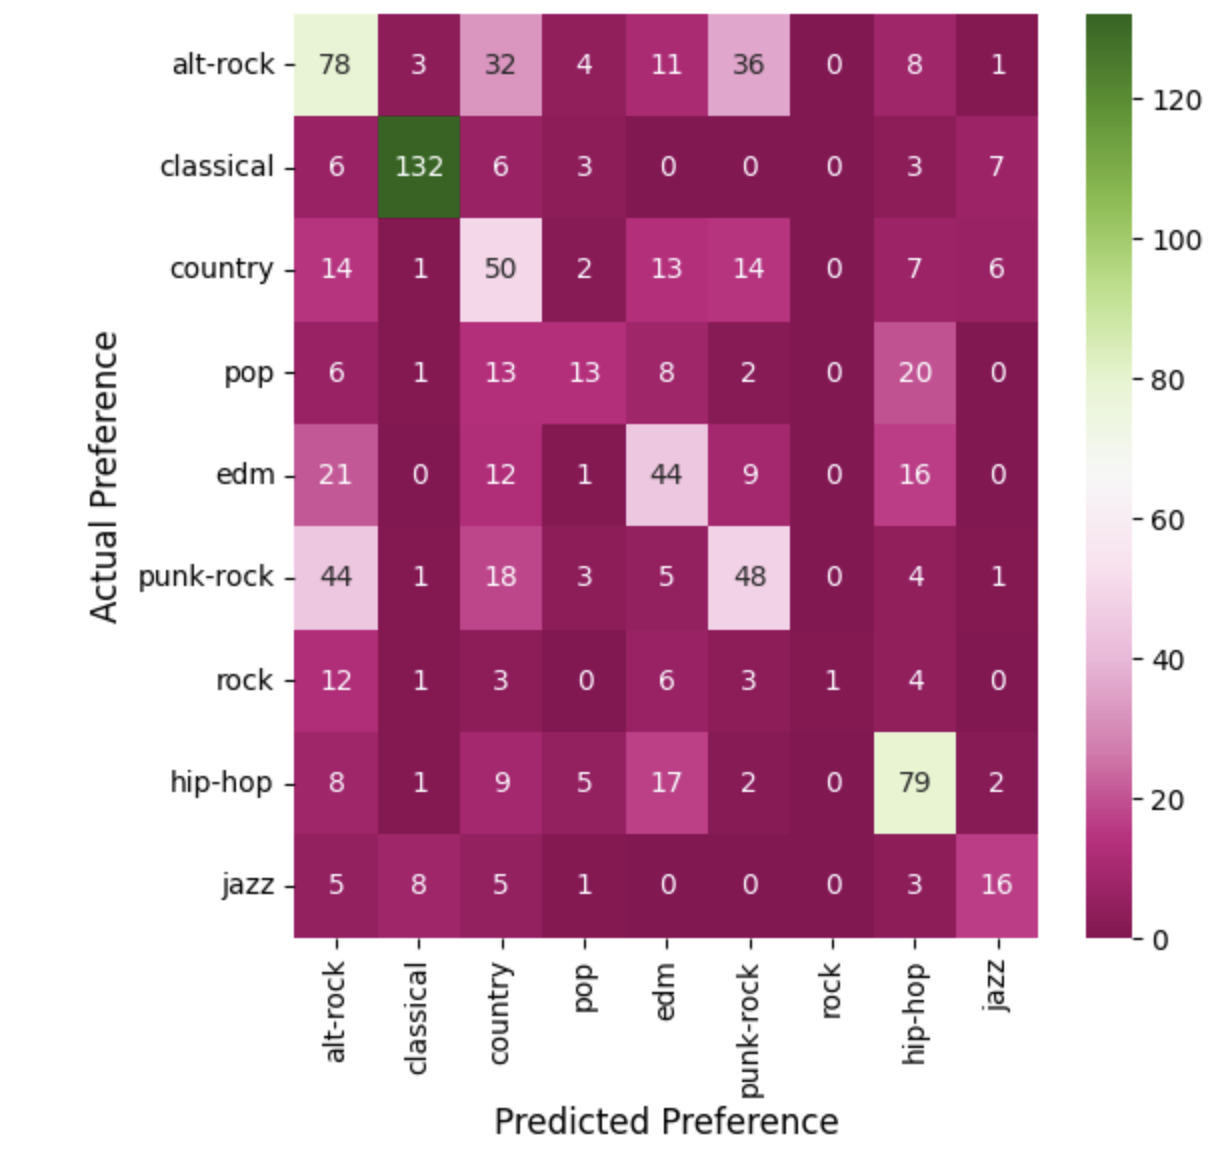
\includegraphics[width=1.0\linewidth]{RFconf_mat.png}
    \caption{Confusion Matrix summarizing the predictions of the Random Forest model; used to identify TP, TN, FP, FN values}
    \label{rf_confmatrix}
\end{figure}

\subsection{KNN}
\subsubsection{Assumption}
\begin{itemize}
    \item \textbf{Best K Value}: The performance of the KNN model was evaluated by varying the number of neighbors (k) to 20, 40, 60, 80, and 100 on a dataset containing approximately 250,000 entries.
    \item \textbf{Performance Metrics}: The accuracy, precision, recall, and F1 score of each model were compared based on the confusion matrix.
    \item \textbf{Genre Analysis}: The dataset includes 9 genres. Macro averages are compared for each genre. It is important to note that the micro averages for accuracy, precision, recall, and F1 score will be the same. There is a significant disparity in the sample sizes of each genre, with differences up to six times, suggesting that macro averages might not accurately reflect the model's performance.
    \item \textbf{K-fold Cross Validation}: To mitigate the impact of sample size disparities among genres --- Depending on data splitting, samples of certain genres may be largely absent from the training data ---, K-fold cross-validation was applied to the training data, split at 80:20. The performance metrics for each fold were averaged to represent the accuracy of the KNN model for each number of neighbors (k). Note that the best performance was not adopted; instead, the average performance across folds was used.
    \item \textbf{Top-t Assumption}:
    \begin{itemize}
        \item Single genre prediction results in low accuracy. To mitigate this, the top \verb|t| genres with the highest counts among the nearest neighbors are considered as the prediction. The accuracy is then measured based on whether the true genre of the test track is included within these top \verb|t| predicted genres.
        \item Naturally, as the value of \verb|t| increases, the coverage improves, leading to higher accuracy. However, this also reduces the strictness of the prediction. Therefore, accuracy weighted by \verb|t| is used for comparison.
        \item The weighting is done using $e^{-t/N}$, where $N$ is the total number of genres, which is 9 in our dataset.
    \end{itemize}
\end{itemize}

\subsubsection{Best $K$ Value Experiment}
The full results are presented in Table \ref{table:result}.
\begin{table}
    \begin{center}
        \begin{tabular}{|c||c|c|c|c|c|} \hline
           $n$ & accuracy & precision & recall & f1 & time   \\
           \hline
            20  & 0.5299 & 0.5248 & 0.5221 & 0.5213 & 98.71  \\
            40  & 0.5353 & 0.5315 & 0.5244 & 0.5254 & 116.67 \\
            60  & 0.5355 & 0.5324 & 0.5227 & 0.5246 & 130.93 \\
            80  & 0.5347 & 0.5320 & 0.5203 & 0.5228 & 143.82 \\
            100 & 0.5342 & 0.5317 & 0.5187 & 0.5215 & 151.74 \\
            \hline
        \end{tabular}
        \caption{Results for different $n_{neighbors}$. \textit{precision}, \textit{recall}, and \textit{f1} are the macro-averages, respectively.}
        \label{table:result}
    \end{center}
\end{table}
\begin{itemize}
    \item \textbf{Accuracy}: Shown in Figure \ref{fig:accuracy}, the accuracy varies from 0.5299 (k=20) to 0.5355 (k=60). This small range of variation (approximately 0.006) suggests that the model's performance is relatively stable across different values of \verb|n_neighbors|. The accuracy increased as the value of \verb|n_neighbors| approached 60, after which it started to decline. This indicates that the optimal number of neighbors for maximizing accuracy lies around 60.
    \begin{figure}[H]
        \centering
        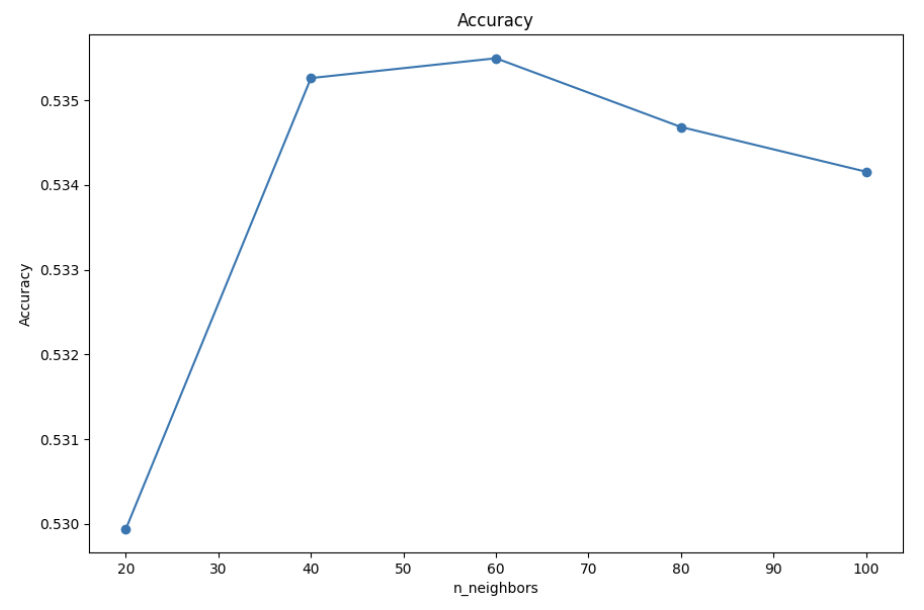
\includegraphics[width=1.0\linewidth]{KNN_Accuracy.png}
        \caption{Accuracy}
        \label{fig:accuracy}
    \end{figure}
    
    \item \textbf{Precision (Macro)}: Shown in Figure \ref{fig:precision}, the macro-averaged precision ranges from 0.5248 (k=20) to 0.5324 (k=60). This suggests that the model's precision across different classes is relatively consistent. The precision increased as the value of \verb|n_neighbors| approached 60, after which it started to decline. This indicates that the optimal number of neighbors for maximizing accuracy lies around 60.
    \begin{figure}[H]
        \centering
        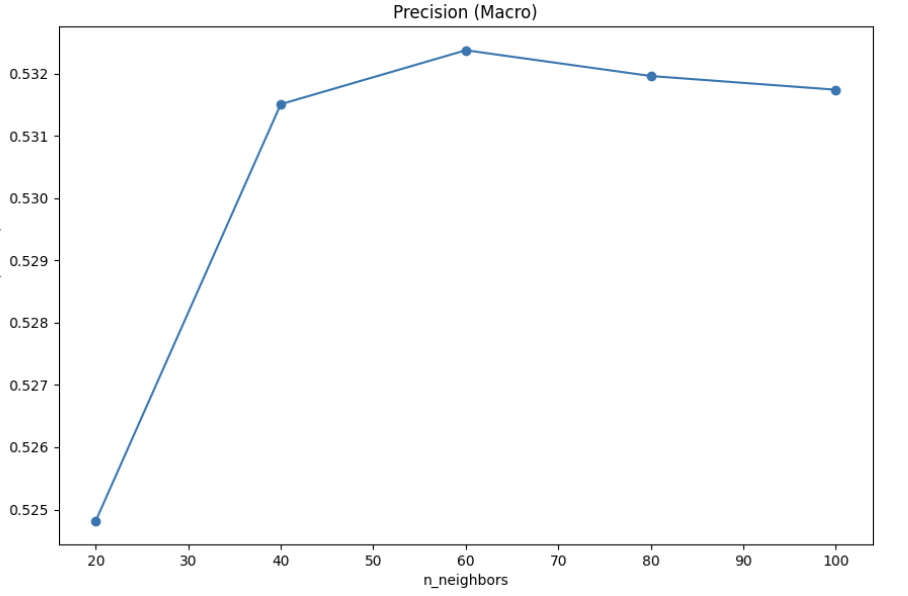
\includegraphics[width=1.0\linewidth]{KNN_precision_macro.png}
        \caption{Macro Average of Precision}
        \label{fig:precision}
    \end{figure}

    \item \textbf{Recall (Macro)}: Shown in Figure \ref{fig:recall}, the macro-averaged recall ranges from 0.5187 (k=100) to 0.5221 (k=20). This indicates that the model's recall across different classes does not vary significantly. In contrast to precision, recall values exhibited a downward trend as the number of neighbors increased. This inverse relationship between precision and recall is typical due to their inherent trade-off.
    \begin{figure}[H]
        \centering
        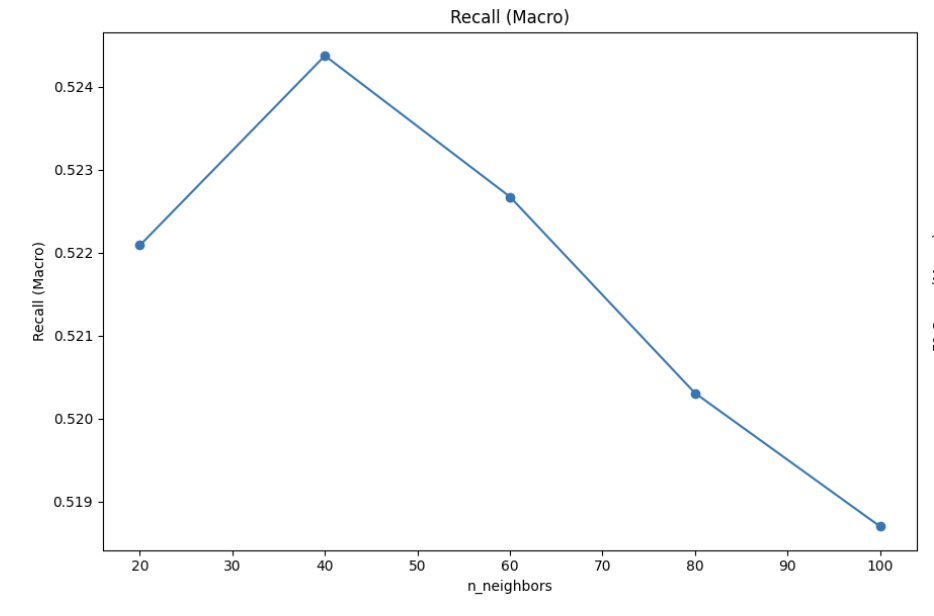
\includegraphics[width=1.0\linewidth]{KNN_recall_macro.png}
        \caption{Macro Average of Recall}
        \label{fig:recall}
    \end{figure}
    
    \item \textbf{F1 Score (Macro)}: Shown in Figure \ref{fig:f1}, the macro-averaged F1 score ranges from 0.5213 (k=20) to 0.5246 (k=60), reflecting a balanced performance across different classes. The F1 score, which balances precision and recall, mirrored the trend observed in accuracy. It increased towards \verb|n_neighbors| = 40 and decreased beyond this point. Thus, the optimal F1 score is also achieved at \verb|n_neighbors| = 40.
    \begin{figure}[H]
        \centering
        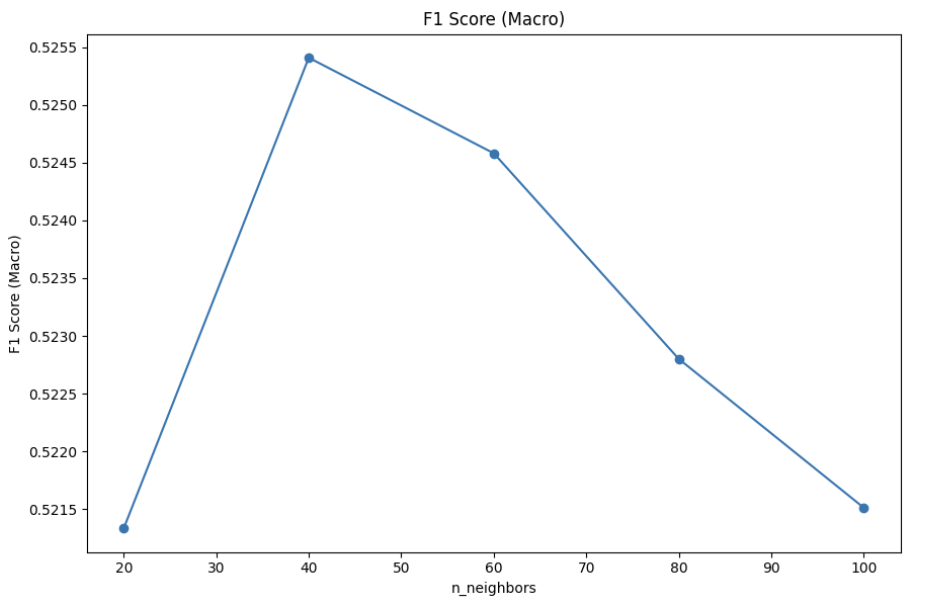
\includegraphics[width=1.0\linewidth]{KNN_F1Score.png}
        \caption{Macro Average of F1 Score}
        \label{fig:f1}
    \end{figure}
\end{itemize}

\textbf{Implication}:
Upon analyzing the trends for each performance metric, it is evident that the variations across different values of $n_{neighbors}$ are relatively small. This indicates that the model's performance remains stable across different neighborhood sizes. However, it is important to note that the values for all metrics hover around 50\%, which suggests that the performance of this classification model is quite low. The stability observed in the model's performance metrics across different neighborhood sizes does not compensate for its overall low accuracy, precision, recall, and F1 scores. Therefore, it can be concluded that while the model's stability is a positive aspect, its effectiveness in classifying genres is limited and requires significant improvement.

\subsubsection{Top-t Experiment}
The experimental results for varying the number of top genres (\verb|t| $\in \{2, 3, \ldots, N-1\}$) are presented in Table \ref{tab:top_t}. Additionally, the trends in accuracy and weighted accuracy are visualized in Figure \ref{fig:top_t_accuracy} and Figure \ref{fig:weighted_top_t_accuracy} respectively.

\begin{table}[h]
    \centering
    \caption{Top K Accuracy and Weighted Accuracy for Different Values of $t$}
    \label{tab:top_t}
    \begin{tabular}{|c||c|c|}
    \hline
    $t$ & Top t Accuracy & Weighted Accuracy \\
    \hline
    2 & 0.7406 & 0.5930 \\
    3 & 0.8428 & 0.6039 \\
    4 & 0.9036 & 0.5794 \\
    5 & 0.9453 & 0.5424 \\
    6 & 0.9718 & 0.4989 \\
    7 & 0.9850 & 0.4525 \\
    8 & 0.9899 & 0.4070 \\
    \hline
    \end{tabular}
\end{table}

\begin{figure}[H]
    \centering
    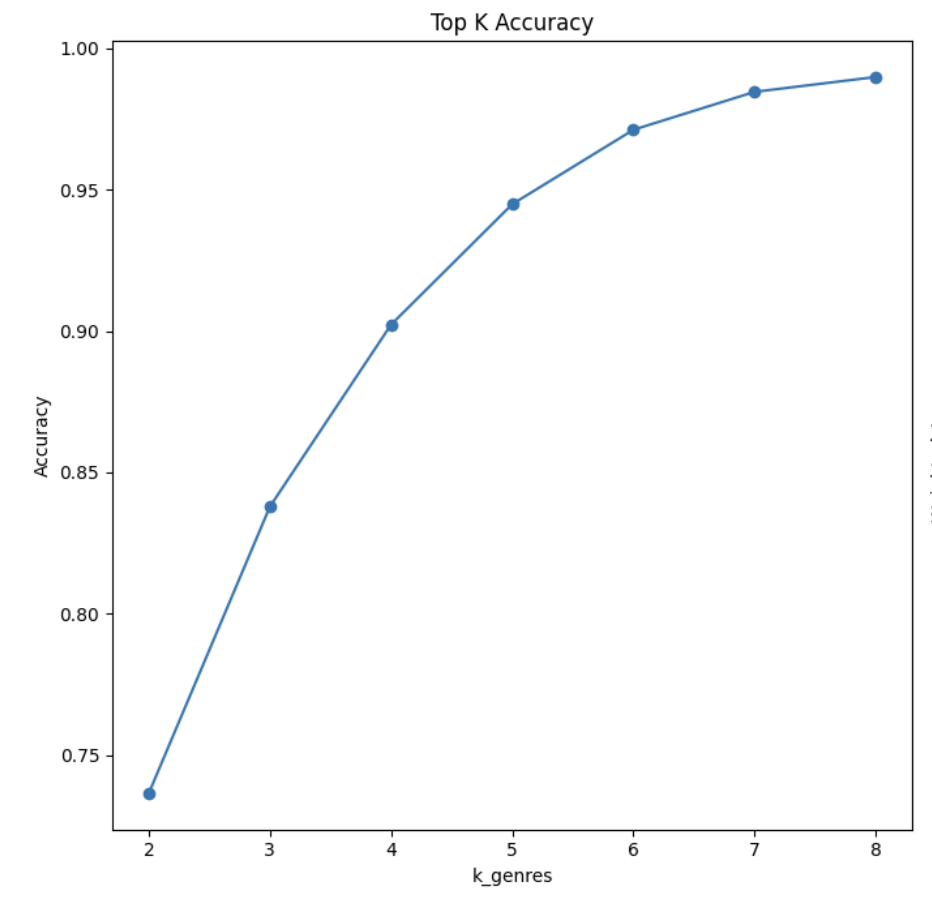
\includegraphics[width=1.0\linewidth]{KNN_Top_K_Accuracy.png}
    \caption{Top t Accuracy}
    \label{fig:top_t_accuracy}
\end{figure}

\begin{figure}[H]
    \centering
    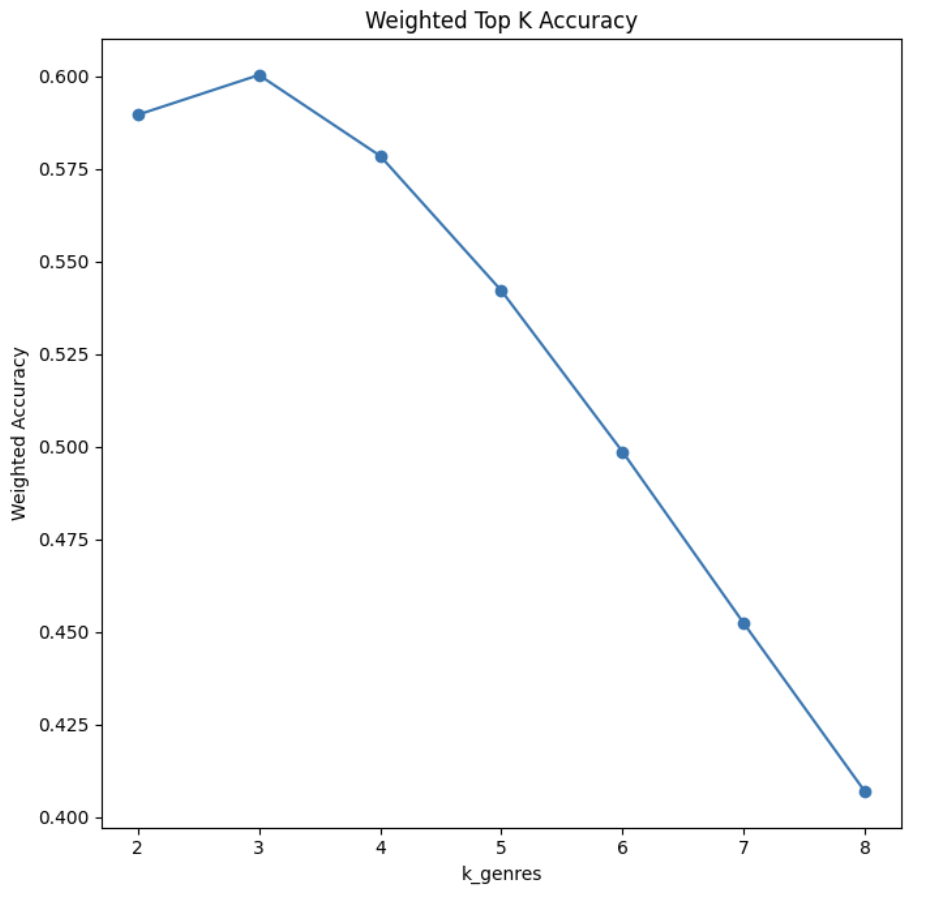
\includegraphics[width=1.0\linewidth]{KNN_weighted_Top_K_Accuracy.png}
    \caption{Weighted Top t Accuracy}
    \label{fig:weighted_top_t_accuracy}
\end{figure}

The results show that as the value of $t$ increases, the Top K Accuracy consistently improves. This is expected, as considering more genres increases the likelihood that the true genre is included in the top predictions. However, the Weighted Accuracy, which incorporates the penalty term $e^{-t/N}$ to account for the reduction in strictness, shows a different trend. The Weighted Accuracy peaks at $t = 3$ and then decreases as $t$ increases. This indicates that while increasing $t$ improves coverage, it also reduces the model's specificity.

\textbf{Implication}:
\begin{itemize}
    \item \textbf{Top t Accuracy} increases with $t$, reaching nearly 99\% when $t = 8$.
    \item \textbf{Weighted Accuracy} peaks at $t = 3$, suggesting that this value balances coverage and specificity most effectively for this dataset.
    \item As $t$ increases beyond 3, the Weighted Accuracy decreases, highlighting the trade-off between including more potential genres and maintaining prediction specificity.
\end{itemize}

These findings underscore the importance of selecting an optimal value for $t$ that balances accuracy and specificity in genre prediction tasks. Certainly, changing the type and parameters of the weight function will change the optimal $t$, but exponential weights, where the decay in accuracy increases as $t$ increases, are suitable, and the value $t=3$ seems reasonable.

\section{Conclusion}
The model demonstrates stable performance across different values of $n_{neighbors}$, indicating its robustness in genre classification tasks. However, despite this stability, the overall performance remains relatively low, suggesting the need for further improvements.

Based on the analysis, \verb|n_neighbors| = 60 was determined to be the optimal number of neighbors for the KNN model. Precision (macro) peaks at \verb|n_neighbors| = 60, while recall and F1 score peak at \verb|n_neighbors| = 40. Accuracy also peaks at \verb|n_neighbors| = 60. Although recall and F1 score peak at a different value, the nature of the genre classification task suggests that false negatives (FN) have a smaller impact. Therefore, higher precision is prioritized in this context. Given that precision (macro) peaks at \verb|n_neighbors| = 60, this value is considered the optimal setting for the KNN model in this study.

To compensate for the low overall accuracy of the model, the number of genres presented as predictions was increased. This approach involves considering the top T genres with the highest counts among the nearest neighbors as potential predictions. By doing so, the likelihood that the true genre is included in the predictions is increased, thereby improving user experience. However, it is crucial to balance between coverage and specificity, as increasing T improves coverage but reduces prediction strictness. Weighted accuracy, which incorporates a penalty term $e^{-t/N}$, where $N$ is the total number of genres, is used to evaluate the effectiveness of this approach. In our experiments, $t=3$ was found to be the optimal value. Therefore, when applying this model for genre classification, it is expected to present the top 3 genres as predictions.

\section{Discussion}
When evaluating the performance of Random Forest and k-Nearest Neighbors for classifying song genre based on individual characteristics of the song, the resulting model indicated that it is possible to predict the genre of a song based on these features, however there was a consistently low accuracy across the attempted models. Since both models had relatively low accuracy, we decided that k-Nearest Neighbors would be the ideal choice, as it would output more than one genre prediction for each song. In regards to potential improvements, one limiting factor that we found with our dataset was that genres of Spotify songs are generally assigned based on the artist, rather than the song itself. For example, every song by Olivia Rodrigo is listed as pop, despite songs such as “good 4 u” and “brutal” being largely classified as alternative rock or pop-punk by the media and mainstream audience. This adversely affected the model during the training process since track features correlated with rock songs might be labeled as pop, thus potentially making both rock and pop predictions less accurate during testing. Instead, using a dataset where genre is assigned to individual songs, would increase model accuracy, as the classified genre would be more accurately based on these features specific to the song. We would also explore less computationally expensive methods, as although we found k-Nearest Neighbors to be an effective model for this multi-class classification, it became increasingly time-consuming to process the large training data set, requiring a large k parameter. 

\section{Github link and Project Roadmap}

\section{Works Cited}
\printbibliography


\end{document}
